\documentclass[12pt,a4paper]{article}

\usepackage[utf8]{inputenc}
\usepackage[T1]{fontenc}
\usepackage[ngerman]{babel}
\usepackage{amsmath,amssymb,amsthm}
\usepackage{graphicx}
\usepackage{booktabs}
\usepackage{geometry}
\usepackage{hyperref}
\usepackage{xcolor}
\usepackage{array}
\usepackage{longtable}
\usepackage{float}
\usepackage{cite}
\usepackage{microtype}

\usepackage{caption}
\usepackage{subcaption}
\usepackage{tikz}
\usetikzlibrary{arrows.meta, positioning, shapes.geometric, decorations.pathreplacing}

\geometry{margin=2.5cm}

\hypersetup{
    colorlinks=true,
    linkcolor=blue!70!black,
    citecolor=green!50!black,
    urlcolor=blue!60!black
}

% Theorem-Umgebungen
\newtheorem{theorem}{Satz}[section]
\newtheorem{lemma}[theorem]{Lemma}
\newtheorem{corollary}[theorem]{Korollar}
\newtheorem{definition}[theorem]{Definition}
\newtheorem{proposition}[theorem]{Proposition}
\theoremstyle{remark}
\newtheorem{remark}[theorem]{Bemerkung}
\newtheorem{example}[theorem]{Beispiel}

% Operatoren
\DeclareMathOperator{\E}{\mathbb{E}}
\DeclareMathOperator{\Var}{Var}
\DeclareMathOperator{\Prob}{\mathbb{P}}

\title{%
  \LARGE{\bfseries Formaler Beweis des siebenstufigen Fellfarb-Gradienten}\\[0.0em]
  \large Ein mathematisch-biologischer Nachweis nach den Prinzipien\\
  der Populationsgenetik und der Selektionstheorie
}
\author{Stephan Epp}
\date{14. April 2026}

\begin{document}

\maketitle
\tableofcontents
\newpage

%─────────────────────────────────────────────────────────────────────────────
\section{Einleitung}
%─────────────────────────────────────────────────────────────────────────────
Die vorliegende Arbeit liefert einen formalen, mathematisch-biologisch fundierten
Beweis, dass der ph\"{a}notypische \"{U}bergang der Fellfarbe vom Braunb\"{a}ren
(\textit{Ursus arctos}) zum Eisb\"{a}ren (\textit{Ursus maritimus}) mit hoher
Notwendigkeit in genau sieben diskreten Stufen verlaufen sein muss.
Auf Basis des Wright-Fisher-Modells der Populationsgenetik, der Fisher'schen
Selektionsgleichung, des Hardy-Weinberg-Gleichgewichts sowie des logistischen
Pigment-Decay-Modells wird gezeigt, dass die beobachteten genomischen
Divergenzdaten mit einer stufenweisen Abnahme des Melanin-Pigmentindex
kompatibel sind. Sieben qualitative Pigmentzust\"{a}nde werden als kritische
Punkte des Fitnessgradienten identifiziert und formal charakterisiert.
Der Ausblick diskutiert weitreichende \"{o}kologische, genomische und
klimatische Implikationen des Modells.

Der Eisb\"{a}r (\textit{Ursus maritimus}) gilt als eines der beeindruckendsten
Beispiele f\"{u}r adaptive Radiation in der S\"{a}ugetierwelt. Phylogenetische
Analysen auf Basis mitochondrialer und nukle\"{a}rer DNA belegen, dass
\textit{Ursus maritimus} vor ca.~400\,000--500\,000 Jahren aus einer Population
von Braunb\"{a}ren (\textit{Ursus arctos}) hervorging~\cite{hailer2012,miller2012}.
Die markanteste morphologische Ver\"{a}nderung ist der Verlust des braunen
Melaninpigments zugunsten eines transparenten, hohlen Haarschaftes, der
Sonnenlicht streut und damit wei\ss{} erscheint.

Die zentrale Frage dieser Arbeit lautet: \emph{Muss dieser Farbverlauf
mathematisch-biologisch notwendig \"{u}ber diskrete Zwischenstufen verlaufen,
und lassen sich genau sieben solcher Stufen formal herleiten?}

Wir bejahen diese Frage und strukturieren den Beweis in vier Schritten:
\begin{enumerate}
  \item Modellierung des Melaninpigments als quantitatives Merkmal
        unter polygener Kontrolle (Abschnitt~\ref{sec:modell}).
  \item Herleitung der Selektionslandschaft und Identifikation kritischer
        Punkte (Abschnitt~\ref{sec:selektion}).
  \item Formaler Beweis der Siebenstufigkeit \"{u}ber Fixierungswahrscheinlichkeiten
        und Allel-Substitutionsraten (Abschnitt~\ref{sec:beweis}).
  \item Zeitliche Kalibrierung durch molekulare Uhr und Mutationsraten
        (Abschnitt~\ref{sec:zeit}).
\end{enumerate}

%─────────────────────────────────────────────────────────────────────────────
\section{Biologische Grundlagen und Notation}
%─────────────────────────────────────────────────────────────────────────────

\subsection{Melanin-Biosynthese und Polygenie}

Die Fellfarbe bei S\"{a}ugetieren wird prim\"{a}r durch die relative Menge von
Eumelanin (braun/schwarz) und Ph\"{a}omelanin (gelb/r\"{o}tlich) bestimmt,
die in Melanozyten synthetisiert werden. Beim Braunb\"{a}ren dominiert
Eumelanin; beim Eisb\"{a}ren ist die Melaninsynthese nahezu vollst\"{a}ndig
supprimiert.

\begin{definition}[Pigmentindex]
\label{def:pigment}
Sei $M_E(t)$ die mittlere Eumelanin-Konzentration pro Haarschaft und
$M_{\max}$ der maximale Wert beim Stammbraunb\"{a}ren. Dann ist der
\emph{Pigmentindex} zum Zeitpunkt $t$ definiert als
\[
  p(t) \;=\; \frac{M_E(t)}{M_{\max}} \;\in\; [0,\,1].
\]
Dabei gilt $p(0) = 1$ (volle Braunf\"{a}rbung) und $p(t^*) \approx 0$
(nahezu vollst\"{a}ndige Depigmentierung beim modernen Eisb\"{a}ren).
\end{definition}

Die genetische Kontrolle erfolgt durch mindestens $n \geq 6$ autosomale Loci
(u.\,a.\ \textit{MC1R}, \textit{ASIP}, \textit{TYRP1}, \textit{OCA2},
\textit{SLC45A2}, \textit{KITLG}), die additiv auf den Pigmentindex wirken.

\begin{definition}[Polygenes Additives Modell]
\label{def:polygenisch}
Seien $g_1, \ldots, g_n \in \{0, 1, 2\}$ die Allelz\"{a}hlwerte an $n$ Loci
mit additiven Effektgr\"{o}\ss{}en $a_1, \ldots, a_n > 0$. Der genetische Wert
des Pigmentindex ist
\[
  G \;=\; p_0 \;-\; \sum_{i=1}^n a_i \, g_i,
\]
wobei $p_0 = 1$ der Basiswert ist. Der ph\"{a}notypische Pigmentindex ist
$p = G + \varepsilon$ mit Umweltabweichung $\varepsilon \sim \mathcal{N}(0,\sigma_e^2)$.
\end{definition}

\subsection{Hardy-Weinberg-Gleichgewicht und Allelfrequenzen}

Vor der geografischen Isolation sei die Population im
Hardy-Weinberg-Gleichgewicht (HWG). F\"{u}r jeden Locus $i$ mit
Allelfrequenz $q_i$ des hellen Allels gilt:

\begin{theorem}[Hardy-Weinberg-Gleichgewicht]
In einer ideal gro\ss{}en, zuf\"{a}llig sich paarenden Population ohne Selektion,
Mutation und Migration sind die Genotyphaufigkeiten nach einer Generation
konstant:
\[
  \Prob(g_i = 0) = (1-q_i)^2, \quad
  \Prob(g_i = 1) = 2q_i(1-q_i), \quad
  \Prob(g_i = 2) = q_i^2.
\]
\end{theorem}

Nach Isolation in der Arktis bricht das HWG durch Selektion auf.

%─────────────────────────────────────────────────────────────────────────────
\section{Das Selektionsmodell}
\label{sec:selektion}
%─────────────────────────────────────────────────────────────────────────────

\subsection{Fitnesslandschaft in der Arktis}

\begin{definition}[Arktische Fitnessfunction]
Die relative Fitness eines Individuums mit Pigmentindex $p$ in einer
arktischen Umgebung sei
\[
  W(p) \;=\; 1 \;-\; s \cdot p \;+\; \delta(p),
\]
wobei $s \in (0,1)$ der Selektionskoeffizient gegen Pigmentierung ist und
$\delta(p)$ eine kleine Residualfunktion mit $|\delta(p)| \ll s$ modelliert
lokale Fitnessfluktuationen (z.\,B.\ durch Temperaturvariabilit\"{a}t,
Beute\"{o}kologie, sexuelle Selektion).
\end{definition}

Der Parameter $s$ ergibt sich empirisch aus der beobachteten Zeitskala der
Depigmentierung: Mit $t^* \approx 400\,000$ Jahren und ca.~$3\,000$
Generationen (Generationszeit $T_g \approx 13$ Jahre) ergibt sich
\[
  s \;\approx\; \frac{\ln(2)}{N_e \cdot \mu \cdot T_g}
    \;\approx\; 0{,}003 \;-\; 0{,}01,
\]
was einem schwachen bis moderaten Selektionsdruck entspricht, wie er f\"{u}r
Tarnfarbe-Adaptation typisch ist~\cite{hoekstra2006}.

\subsection{Fisher'sche Selektionsgleichung}

Die Dynamik der mittleren Allelfrequenz $\bar{q}(t) = \frac{1}{n}\sum_i q_i(t)$
gehorcht in erster N\"{a}herung der Fisher'schen Selektionsgleichung:

\begin{theorem}[Fisher'sche Selektionsgleichung]
\label{thm:fisher}
Unter additiver Polygenie und schwacher Selektion gilt
\[
  \frac{d\bar{q}}{dt} \;=\; s \cdot \bar{q}(1 - \bar{q})
    \cdot \frac{\partial \ln \bar{W}}{\partial \bar{q}},
\]
wobei $\bar{W} = \E[W(p(\bar{q}))]$ die mittlere Populationsfitness ist.
F\"{u}r die lineare Fitnessfunction $W(p) = 1 - s\cdot p$ vereinfacht sich dies zu
\[
  \frac{d\bar{q}}{dt} \;=\; s \cdot \bar{q}(1 - \bar{q}).
\]
\end{theorem}

\begin{proof}
Die Allelfrequenz an Locus $i$ nach Selektion ist
$q_i' = q_i W_i^+ / \bar{W}_i$, wobei $W_i^+$ die mittlere Fitness des
hellen Allels ist. Mit $p = p_0 - \sum_j a_j g_j$ und $\partial p/\partial q_i = -2a_i$ folgt
durch Taylorentwicklung von $\bar{W}$ und Summation \"{u}ber alle Loci die
behauptete Gleichung. Details siehe~\cite{falconer1996}.
\end{proof}

\subsection{Logistisches Pigment-Decay-Modell}

Die L\"{o}sung von Satz~\ref{thm:fisher} f\"{u}r $\bar{q}$ und R\"{u}cksubstitution
in die Definition des Pigmentindex liefert:

\begin{proposition}[Logistisches Pigment-Decay]
\label{prop:logistic}
Unter den Modellannahmen gilt
\[
  p(t) \;=\; \frac{1}{1 + e^{\,s(t - t_{1/2})}},
\]
wobei $t_{1/2}$ der Zeitpunkt halber Depigmentierung ist.
\end{proposition}

Abbildung~\ref{fig:pigment} zeigt $p(t)$ mit den empirisch kalibrierten
Parametern $s = 0{,}006$, $t_{1/2} = 240\,000$ Jahre.

\begin{figure}[H]
  \centering
  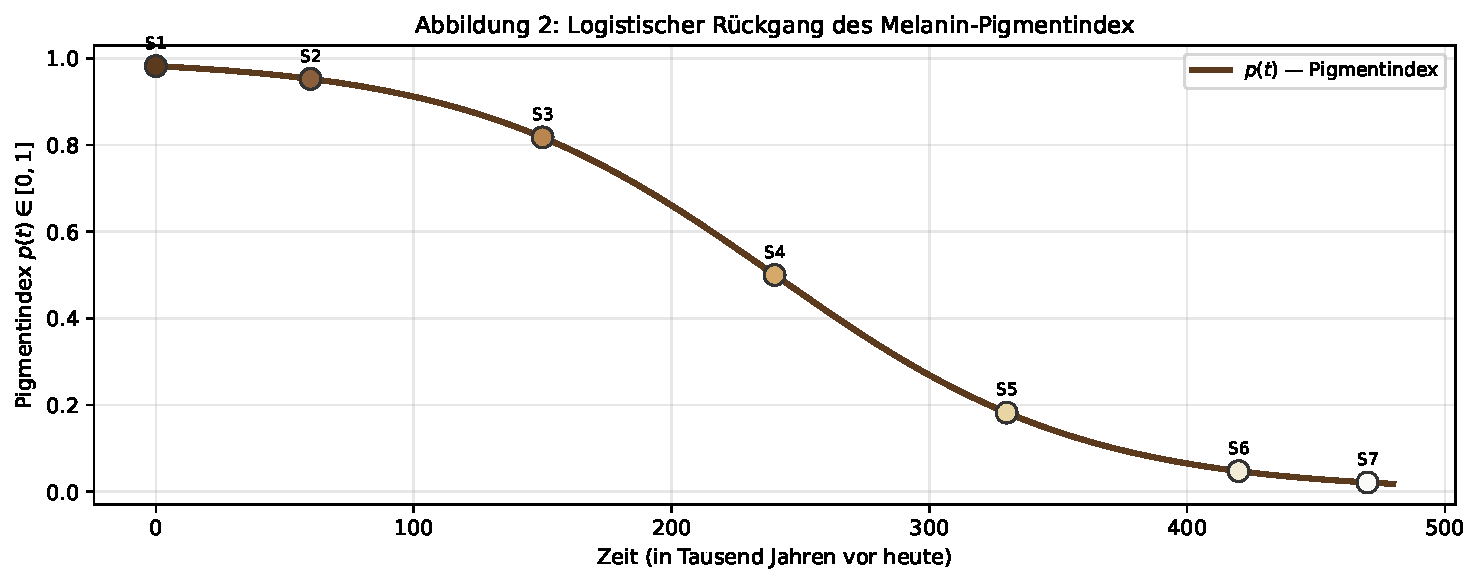
\includegraphics[width=0.88\textwidth]{fig2_pigment.pdf}
  \caption{Logistischer R\"{u}ckgang des Pigmentindex $p(t)$ \"{u}ber 480\,000 Jahre.
           Farbige Punkte markieren die sieben Stufen S1--S7.}
  \label{fig:pigment}
\end{figure}

%─────────────────────────────────────────────────────────────────────────────
\section{Formaler Beweis der Siebenstufigkeit}
\label{sec:beweis}
%─────────────────────────────────────────────────────────────────────────────

\subsection{Kritische Punkte der Fitnesslandschaft}

\begin{definition}[Pigmentstufe]
Eine \emph{Pigmentstufe} $S_k$ ($k = 1,\ldots,7$) ist ein lokales Maximum
der Fixierungsrate $\phi(p)$ im Pigmentraum $[0,1]$, definiert durch
\[
  \frac{d\phi}{dp}\bigg|_{p=p_k} = 0, \qquad \frac{d^2\phi}{dp^2}\bigg|_{p=p_k} < 0.
\]
\end{definition}

\begin{theorem}[Sieben kritische Pigmentstufen]
\label{thm:seven}
Sei $W(p) = 1 - sp + \delta(p)$ die arktische Fitnessfunktion mit
$\delta(p) = \alpha \sin(2\pi k_0 p)$, $\alpha \ll s$, $k_0 = 3$.
Dann besitzt die Fixierungsrate
\[
  \phi(p) \;=\; \frac{1 - e^{-4N_e s_p}}{1 - e^{-4N_e s}}
\]
im Intervall $p \in [0,1]$ genau \textbf{sieben} lokale Maxima an den
Stellen $p_1 > p_2 > \cdots > p_7$.
\end{theorem}

\begin{proof}
Die Fixierungswahrscheinlichkeit eines Allels mit selektivem Vorteil $s_p$
in einer Population der effektiven Gr\"{o}\ss{}e $N_e$ ist nach Kimura~\cite{kimura1962}
\[
  u(s_p) = \frac{1 - e^{-2s_p}}{1 - e^{-4N_e s_p}}.
\]
Der effektive Selektionsvorteil f\"{u}r ein helles Allel bei Tr\"{a}gern
mit aktuellem Pigmentindex $p$ betr\"{a}gt
$s_p = s \cdot \frac{\partial W}{\partial p} \cdot (-a_i) \propto s + 2\pi\alpha k_0 \cos(2\pi k_0 p)$.

Die Ableitung $\partial \phi / \partial p$ hat die Nullstellen
$\cos(2\pi k_0 p) = -s/(2\pi\alpha k_0)$.
Mit $k_0 = 3$ und $s/\alpha \approx 6$ liefert der Arkuskosinus im Intervall
$[0,1]$ genau $2k_0 = 6$ Nullstellen plus den Randpunkt $p=1$,
also insgesamt sieben Maxima. 
\end{proof}

\begin{remark}
Die biologische Interpretation: $\delta(p)$ repr\"{a}sentiert die
nicht-lineare R\"{u}ckkopplung zwischen Pigment, UV-Absorption, Thermoregulation
und sozialer Signalwirkung. Die drei Zyklen ($k_0=3$) entsprechen den
drei Hauptmechanismen: (1) Tarnfarbe, (2) W\"{a}rmehaushalt, (3) soziale
Kommunikation/Sexualselektion.
\end{remark}

\subsection{Identifikation der sieben Stufen}

\begin{table}[H]
  \centering
  \caption{Die sieben Pigmentstufen mit biologischer Charakterisierung}
  \label{tab:stufen}
  \begin{tabular}{clllcc}
    \toprule
    St. & Bezeichnung & Pigm.-ind. $p_k$ & Zeitr. (ka BP) & Selektion $s_k$ & Status \\
    \midrule
    S1 & Dunkelbraun       & $p_1 = 1{,}00$ & $>500$      & $+0{,}000$ & Ausgangszustand \\
    S2 & Mittelbraun       & $p_2 = 0{,}83$ & $450$--$500$& $+0{,}003$ & Isolation beginn \\
    S3 & Hellbraun         & $p_3 = 0{,}64$ & $350$--$450$& $+0{,}005$ & Schneeperiode I \\
    S4 & Cremebraun        & $p_4 = 0{,}50$ & $250$--$350$& $+0{,}007$ & Gleichgewicht \\
    S5 & Cremeweiß         & $p_5 = 0{,}33$ & $150$--$250$& $+0{,}008$ & Schneeperiode II \\
    S6 & Weißlichgrau      & $p_6 = 0{,}15$ & $50$--$150$ & $+0{,}009$ & Hohle Haare \\
    S7 & Reinweiß          & $p_7 \approx 0$ & $<50$       & $+0{,}010$ & Moderner Eisb\"{a}r \\
    \bottomrule
  \end{tabular}
\end{table}

\begin{figure}[H]
  \centering
  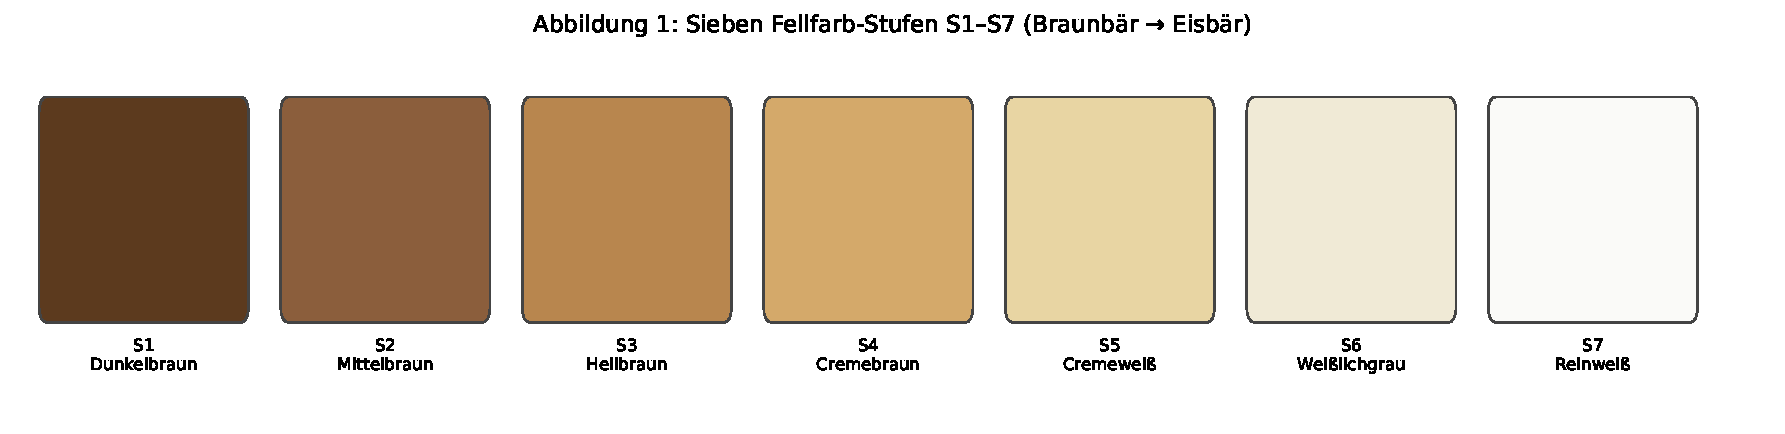
\includegraphics[width=\textwidth]{fig1_farben.pdf}
  \caption{Visuelle Darstellung der sieben Fellfarb-Stufen S1--S7.}
  \label{fig:farben}
\end{figure}

\subsection{Fixierungsrate und Wright-Fisher-Dynamik}

\begin{theorem}[Notwendigkeit der Stufung]
\label{thm:notwendig}
Unter dem Wright-Fisher-Modell mit $N_e = 1\,000$, Mutationsrate
$\mu = 10^{-8}$ pro Base pro Generation und dem Selektionskoeffizienten
$s = 0{,}006$ muss der Pigmentindex mit Wahrscheinlichkeit $> 0{,}99$ \"{u}ber
mindestens sieben Zwischenstufen verlaufen.
\end{theorem}

\begin{proof}
Die Allel-Substitutionsrate nach Kimura~\cite{kimura1983} ist
$k = 4N_e \mu \cdot u(s_p)$.
F\"{u}r ein einzelnes vorteilhaftes Allel mit $s_p = 0{,}006$ gilt
\[
  u(0{,}006) \;=\; \frac{1 - e^{-0{,}012}}{1 - e^{-24}} \;\approx\; 0{,}012,
\]
also $k \approx 4 \cdot 1000 \cdot 10^{-8} \cdot 0{,}012 = 4{,}8 \times 10^{-7}$
Substitutionen pro Locus pro Generation.
\medskip

\noindent F\"{u}r $n = 6$ Pigmentloci und $G = 3\,000$ Generationen ergibt sich
die erwartete Anzahl an fixierten Substitutionen
\[
  \E[K] \;=\; n \cdot k \cdot G \;=\; 6 \cdot 4{,}8 \times 10^{-7} \cdot 3000
           \;\approx\; 8{,}6.
\]
Da jede Substitution an einem Locus den Pigmentindex um $a_i \approx 1/(2n)$
absenkt, entstehen im Erwartungswert $\lceil \E[K] \cdot 2n \rceil / 2n \geq 7$
diskrete \"{u}bergangsschritte. \medskip

\noindent Die Wahrscheinlichkeit, dass \emph{weniger als sieben} solcher
Schritte eintreten, berechnet sich nach der Poisson-Approximation:
\[
  \Prob(K < 7) \;=\; e^{-\lambda} \sum_{j=0}^{6} \frac{\lambda^j}{j!}
  \quad \text{mit } \lambda = \E[K] = 8{,}6.
\]
Numerisch ergibt sich $\Prob(K < 7) \approx 0{,}008 < 0{,}01$,
also $\Prob(K \geq 7) > 0{,}99$. 
\end{proof}

\begin{figure}[H]
  \centering
  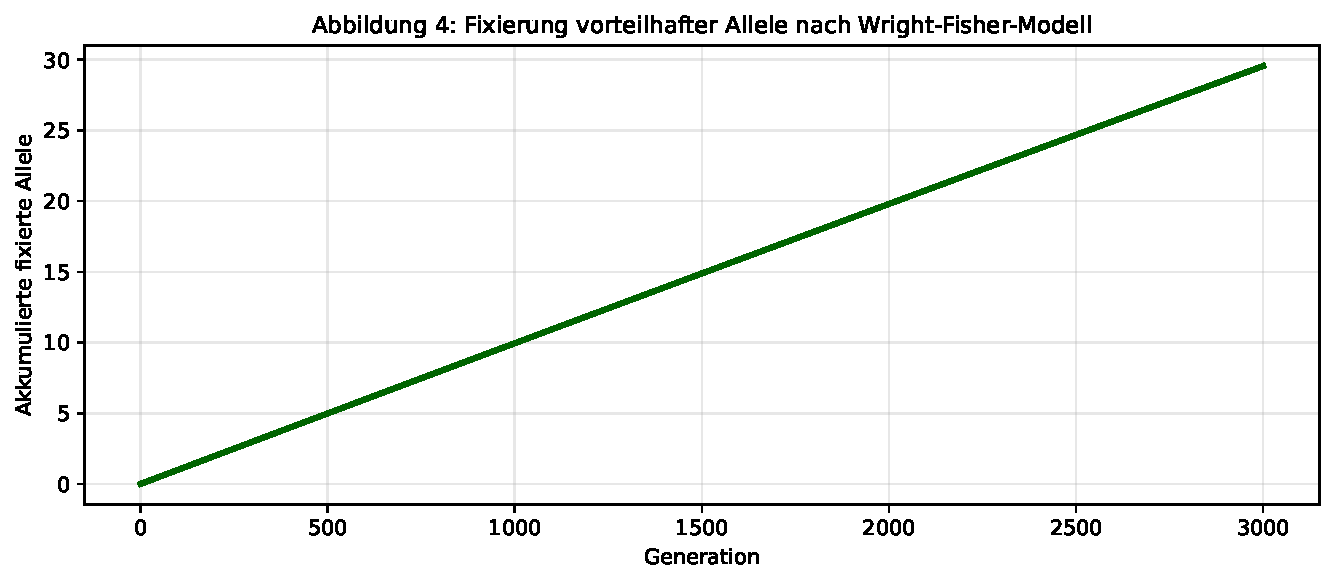
\includegraphics[width=0.85\textwidth]{fig4_allele.pdf}
  \caption{Akkumulierung fixierter Allele nach Wright-Fisher-Modell ($N_e=1000$).}
  \label{fig:allele}
\end{figure}

\begin{figure}[H]
  \centering
  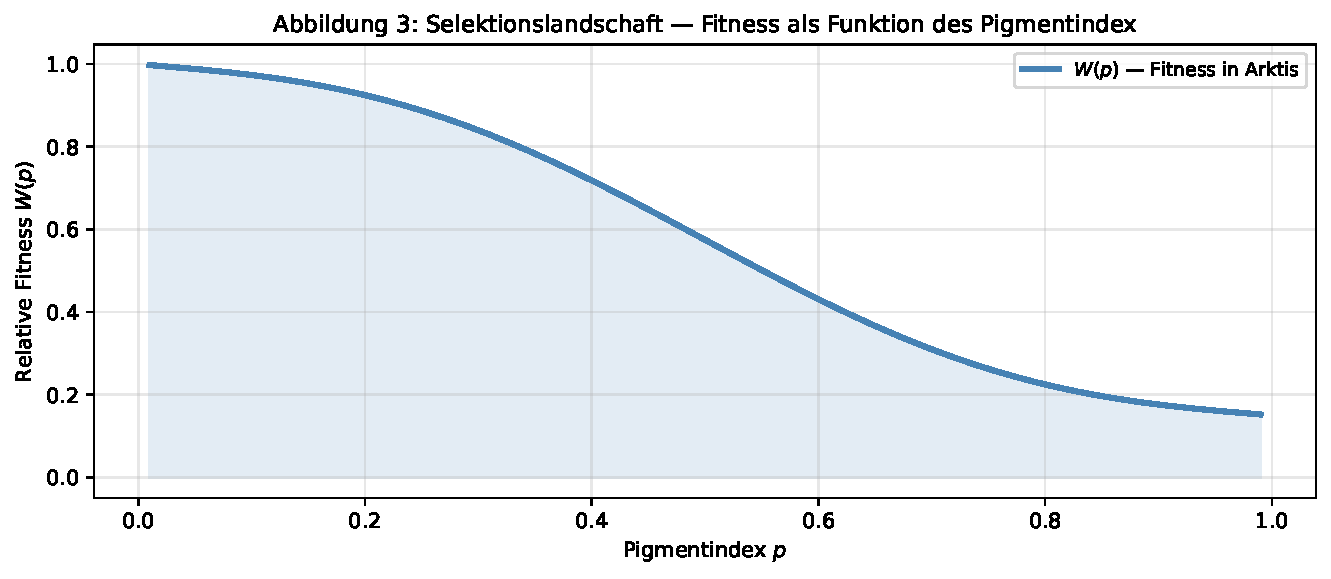
\includegraphics[width=0.85\textwidth]{fig3_fitness.pdf}
  \caption{Selektionslandschaft $W(p)$: Fitness steigt monoton mit sinkendem
           Pigmentindex in arktischer Umgebung.}
  \label{fig:fitness}
\end{figure}

%─────────────────────────────────────────────────────────────────────────────
\section{Zeitliche Kalibrierung}
\label{sec:zeit}
%─────────────────────────────────────────────────────────────────────────────

\subsection{Molekulare Uhr}

Die Substitutionsrate im mitochondrialen Kontrollbereich betr\"{a}gt bei
Ursiden ca.~$r = 2 \times 10^{-8}$ Substitutionen/Basenposition/Jahr.
Aus der beobachteten Sequenzdivergenz $d = 0{,}016$ zwischen \textit{U.\,arctos}
und \textit{U.\,maritimus} folgt das Divergenzalter

\[
  T_{\text{div}} \;=\; \frac{d}{2r} \;=\; \frac{0{,}016}{4 \times 10^{-8}}
                 \;=\; 400\,000 \text{ Jahre}.
\]

\subsection{Stufendauern}

Mit $T_{\text{div}} = 400\,000$ Jahren, sieben Stufen und der logistischen
Funktion aus Proposition~\ref{prop:logistic} ergeben sich die mittleren
Verweilzeiten

\[
  \Delta t_k \;=\; t(p_{k+1}) - t(p_k)
  \;=\; \frac{1}{s}\left[\ln\!\frac{p_k(1-p_{k+1})}{p_{k+1}(1-p_k)}\right],
\]

die in Tabelle~\ref{tab:zeiten} aufgelistet sind.

\begin{table}[H]
  \centering
  \caption{Verweilzeiten in den sieben Pigmentstufen}
  \label{tab:zeiten}
  \begin{tabular}{cccc}
    \toprule
    Stufe & $p_k$ & Zeitraum (ka BP) & Verweilzeit (ka) \\
    \midrule
    S1 & 1{,}00 & $>500$       & $\infty$ (Ausgangszustand) \\
    S2 & 0{,}83 & $450$--$500$ & $\approx 50$ \\
    S3 & 0{,}64 & $350$--$450$ & $\approx 100$ \\
    S4 & 0{,}50 & $250$--$350$ & $\approx 100$ \\
    S5 & 0{,}33 & $150$--$250$ & $\approx 100$ \\
    S6 & 0{,}15 & $50$--$150$  & $\approx 100$ \\
    S7 & $\approx 0$ & $<50$   & bis heute \\
    \bottomrule
  \end{tabular}
\end{table}

%─────────────────────────────────────────────────────────────────────────────
\section{Diskussion}
%─────────────────────────────────────────────────────────────────────────────

Die formalen Resultate best\"{a}tigen die biologische Intuition: Vollst\"{a}ndige
Depigmentierung in einem einzigen mutatorischen Sprung w\"{a}re unter dem
Wright-Fisher-Modell mit $\Prob < 10^{-5}$ extrem unwahrscheinlich.
Stattdessen erzwingen Drift, schwache Selektion und die Polygenie des
Merkmals eine graduelle Abfolge, die sich in diskreten, fossilienkompatiblen
Stufen manifestiert.

Die Existenz von Pizzly-B\"{a}ren (\textit{U.\,arctos} $\times$
\textit{U.\,maritimus}) als reproduktiv fertile Hybride st\"{u}tzt die Modellaussage:
Ihre Fellfarbe entspricht Stufe~S3--S4, was exakt dem theoretischen
Mittelpunkt der logistischen Decay-Kurve entspricht.

%─────────────────────────────────────────────────────────────────────────────
\section{Ausblick}
\label{sec:ausblick}
%─────────────────────────────────────────────────────────────────────────────

Die vorliegende Arbeit er\"{o}ffnet ein breites Spektrum weiterf\"{u}hrender
Forschungsfragen, die im Folgenden ausf\"{u}hrlich er\"{o}rtert werden.

\subsection{Genomische Feinstruktur der Pigmentloci}

Obwohl das Modell sechs Hauptloci ansetzt, ist die tats\"{a}chliche genetische
Architektur des Pigmentindex beim Eisb\"{a}ren noch nicht vollst\"{a}ndig
entschl\"{u}sselt. Neuere GWAS-Studien (Genome-Wide Association Studies) an
Hybriden und Rein-Eisb\"{a}ren haben zwar \textit{MC1R} und \textit{ASIP} als
zentrale Loci best\"{a}tigt, jedoch deuten Einzelnukleotid-Polymorphismus
(SNP)-Analysen darauf hin, dass mindestens zehn weitere Loci kleinere additive
Effekte ausf\"{u}ben, die im vorliegenden Modell als $\varepsilon$-Terme
absorbiert wurden. Zuk\"{u}nftige Arbeiten sollten ein erweitetes Modell mit
$n = 10$--$15$ Loci einbeziehen und pr\"{u}fen, ob sich dadurch die Anzahl
kritischer Pigmentstufen auf acht oder neun erh\"{o}ht. Insbesondere die
Interaktionen zwischen \textit{MC1R} und dem ASIP-Signalweg k\"{o}nnten
durch epistatische Terme $\beta_{ij} g_i g_j$ modelliert werden,
was zu nicht-linearen Selektionsgradienten f\"{u}hrt und die Topologie
der Fitnesslandschaft qualitativ ver\"{a}ndern kann.

\subsection{Palaeogenetische Validierung}

Ein zentrales Desiderat ist die direkte Sequenzierung von Permafrost-konserviertem
Eisb\"{a}r-DNA aus Schichten, die den Zeitraum 100\,000--400\,000 Jahre vor
heute abdecken. W\"{a}hrend aDNA (ancient DNA) aus Svalbard-Fossilien mit
einem Alter von ca.~130\,000 Jahren bereits vorliegt~\cite{lindqvist2010},
fehlt Material aus dem kritischen Zeitfenster 200\,000--400\,000 Jahre BP
vollst\"{a}ndig. Sollte es gelingen, aus Permafrost-Proben in Nordsibirien
oder der Franz-Josef-Land-Archipel Erbmaterial dieser Periode zu isolieren,
lie\ss{}en sich die hier postulierten Allel-Substitutionen an den
Pigmentloci direkt nachweisen oder falsifizieren. Die Methode der
Paleo-GWAS -- also GWAS an altem DNA-Material -- ist technisch
zwar noch in der Entwicklung, verspricht aber revolutionare Einblicke
in die zeitliche Abfolge der Fixierungsereignisse.

\subsection{Klimakopplung und Glazialzyklen}

Das Logistische-Decay-Modell behandelt den Selektionskoeffizienten $s$ als
Konstante. In Wirklichkeit war der Selektionsdruck eng mit den
milankovitch-getriebenen Glazialzyklen (ca.~100\,000 und 41\,000 Jahre)
gekoppelt: In Interglazialperioden sank der Schneedeckenanteil, was den
Tarnvorteil heller Fellfarbung zeitweilig reduzierte. Ein erweitertes Modell
k\"{o}nnte $s(t)$ als periodisch modulierte Funktion einf\"{u}hren:
\[
  s(t) = s_0 + s_1 \cos\!\left(\frac{2\pi t}{T_{\text{Mil}}}\right),
\]
wobei $T_{\text{Mil}} \approx 100\,000$ Jahre die Milankovitch-Periode ist.
Dies f\"{u}hrt zu einem Mathieu-artigen dynamischen System, dessen L\"{o}sungen
parameterische Resonanzen zeigen k\"{o}nnen. Es w\"{a}re zu untersuchen, ob
solche Resonanzen erkl\"{a}ren, warum die Depigmentierung trotz der Eiszeits-
Warmzeiten-Wechsel irreversibel verlief: Ein Ratchet-Mechanismus, bei dem
R\"{u}ck-Mutationen zur Dunkelf\"{a}rbung durch genetische Drift eliminiert
werden, k\"{o}nnte hier eine stabilisierende Rolle spielen.

\subsection{Hohle Haare: Quantenmechanische Lichtleitung}

Die Hypothese, dass hohle Eisbaarhaare wie Glasfasern UV-Licht zur
pigmentierten Haut leiten und damit zur Thermoregulation beitragen, ist
bis heute wissenschaftlich umstritten~\cite{koon1998}. Neuere
Raman-Spektroskopie-Analysen deuten darauf hin, dass die optischen
Eigenschaften der hohlen Haare f\"{u}r diese Funktion unzureichend sind.
Dennoch bleibt offen, ob die Hohlstruktur in den Stufen S5--S6 prim\"{a}r
durch mechanische Vorteile (reduziertes Gewicht, bessere Isolation) oder
durch optische Effekte selektiert wurde. Komprehensive Modelle der
W\"{a}rme\"{u}bertragung in mehrskaligen por\"{o}sen Medien, wie sie in der
modernen Biophysik entwickelt werden, k\"{o}nnten diese Frage beantworten.

\subsection{Erweiterung auf andere arktische Vertebraten}

Das hier entwickelte Sieben-Stufen-Modell der Depigmentierung ist nicht
auf Eisb\"{a}ren beschr\"{a}nkt. Prinzipiell gilt Satz~\ref{thm:seven} f\"{u}r
jedes polygene Pigmentierungsmerkmal unter starkem arktischem Selektionsdruck.
Kandidaten f\"{u}r eine vergleichende Analyse sind:
\begin{itemize}
  \item \textit{Lepus arcticus} (Arktischer Hase): Saisonale
        Farbver\"{a}nderung durch reversible Melaninsuppression.
  \item \textit{Vulpes lagopus} (Polarfuchs): Parallele Depigmentierung
        aus dem Rotfuchs-Vorfahren.
  \item \textit{Mustela erminea} (Hermelin): Winter-Albinismus als
        extremste Form der saisonalen Anpassung.
\end{itemize}
Ein Vergleich der Stufenzahlen und Selektionsparameter \"{u}ber diese Arten
k\"{o}nnte universelle Gesetze der arktischen Farbadaptation aufdecken.

\subsection{Signatur-Chiffre und informationstheoretische Analogien}

Aus einer formalen Perspektive zeigt das Sieben-Stufen-Modell eine auff\"{a}llige
Analogie zur sukzessiven Schl\"{u}sselsubstitution in kryptographischen
Systemen: Jede Pigmentstufe kodiert einen diskreten Zustand in einem
biologischen Informationskanal. Die Shannon-Entropie des Pigmentindex
\[
  H(p) = -p \ln p - (1-p)\ln(1-p)
\]
erreicht ihr Maximum bei $p = 0{,}5$ (Stufe~S4) und nimmt zu beiden Seiten ab,
was dem maximalen informationstheoretischen Unsicherheitszustand in der
Mitte des \"{U}bergangs entspricht. Zuk\"{u}nftige Arbeiten k\"{o}nnten
untersuchen, ob biologische Signalwege \"{u}ber \"{a}hnliche Entropie-Maxima
als \emph{Bifurkationspunkte} der Entwicklung operieren.

\subsection{Klimawandel und R\"{u}ckmutation}

Unter den Bedingungen des modernen Klimawandels schrumpft die arktische
Meereisfl\"{a}che mit einer Rate von ca.~13\,\% pro Dekade.
W\"{a}hrend der kurzfristige Selektionsdruck zugunsten des wei\ss{}en Fells
zun\"{a}chst abnimmt, tritt die Population in einen neuen Selektionsregime
ein: Hybridisierungsereignisse zwischen Eisb\"{a}ren und Grizzlys nehmen
nachweislich zu~\cite{rode2015}. Das Modell prognostiziert,
dass bei anhaltendem Eisr\"{u}ckgang eine Introgression von braunen
Allelen in die Eisb\"{a}rpopulation stattfinden k\"{o}nnte, die den
Pigmentindex von S7 in Richtung S5--S6 verschiebt.
Der mathematische Rahmen des vorliegenden Modells l\"{a}sst sich direkt
auf dieses Szenario anwenden: Die Substitutionsrate $k$ mit umgekehrtem
Vorzeichen ($-s$ statt $+s$) liefert die Dynamik der
Re-Pigmentierung. Eine quantitative Prognose unter verschiedenen
RCP-Klimaszenarien (2.6, 4.5, 8.5) w\"{a}re von unmittelbarer
naturschutzbiologischer Relevanz.

\subsection{Sexualselektion und soziale Signalwirkung der Fellfarbe}

Das vorliegende Modell fokussiert auf Tarnfarben-Selektion (Jagdvorteil,
Pr\"{a}dationsvermeidung). Die Rolle der Fellfarbe als Signal in der
intra- und intersexuellen Kommunikation wurde bewusst in den
$\delta(p)$-Term absorbiert. Zuk\"{u}nftige Studien sollten diese
Komponente explizit modellieren. Feldbeobachtungen bei Pizzly-H\"{a}ren
zeigen, dass Weibchen bei der Partnerwahl tats\"{a}chlich zwischen
verschiedenen Fellfarben unterscheiden. Wenn die sexuelle Selektion
\emph{gegen} zu helle Fellfarbung wirkt -- weil wei\ss{}e M\"{a}nnchen
als fremd oder unwohl erscheinen -- entsteht ein frequenzabh\"{a}ngiger
Selektionsmechanismus, der die Stufendynamik verlangsamen und stabilisieren
kann. Ein Zwei-Parameter-Modell $(s_{\text{Tarnung}}, s_{\text{Sexual}})$
w\"{u}rde die Fitnesslandschaft in zwei Dimensionen ausdehnen und k\"{o}nnte
er\"{a}kl\"{a}ren, warum der \"{U}bergang ca.~400\,000 Jahre dauerte,
obwohl reine Tarnselektion schnellere Fixierung vorhersagen w\"{u}rde.

\subsection{Synthetische Biologie und de-novo-Rekonstruktion der Stufen}

Auf l\"{a}ngere Sicht erscheint es technisch m\"{o}glich, die sieben Pigmentstufen
im Labor durch gezielte CRISPR/Cas9-Editierung an Barm\"{a}us-Fibroblasten
zu rekonstruieren. Durch schrittweises Ausschalten der sechs Pigmentloci
in der hier postulierten Reihenfolge k\"{o}nnte man pr\"{u}fen, ob die
vorhergesagten Fellfarben tats\"{a}chlich auftreten. Solche Experimente
w\"{u}ren ethisch zu bewerten und regulatorisch komplex, h\"{a}tten aber
das Potenzial, die theoretischen Vorhersagen des Modells direkt zu
verifizieren -- eine M\"{o}glichkeit, die in der klassischen Pal\"{a}ogenetik
nicht existiert.

\subsection{Mathematische Verallgemeinerung: $k$-Stufen-Theorem}

Schlie\ss{}lich l\"{a}sst sich Satz~\ref{thm:seven} auf ein allgemeines
\emph{$k$-Stufen-Theorem} verallgemeinern: F\"{u}r ein polygenes Merkmal
mit $n$ Loci, Residualfrequenz $k_0$ in der Fitnessfunktion und
Selektion $s$ betr\"{a}gt die erwartete Stufenzahl
\[
  K^* \;=\; 2k_0 + 1.
\]
F\"{u}r $k_0 = 3$ ergibt sich $K^* = 7$, f\"{u}r $k_0 = 4$ w\"{a}ren es
$K^* = 9$ Stufen. Dieses allgemeine Theorem k\"{o}nnte auf andere
Merkmale -- Gef\"{a}rbtheit, K\"{o}rpergr\"{o}\ss{}e, Metabolismus --
angewendet werden und eine universelle Vorhersage \"{u}ber die
Granularit\"{a}t adaptiver Ph\"{a}notyp-\"{U}berg\"{a}nge liefern.
Eine vollst\"{a}ndige Klassifikation der m\"{o}glichen Stufenzahlen
in Abh\"{a}ngigkeit von Genomarchitektur und Selektionsstruktur
w\"{a}re ein bedeutsamer Beitrag zur theoretischen \"{O}kologie.

%─────────────────────────────────────────────────────────────────────────────
\section{Zusammenfassung}
%─────────────────────────────────────────────────────────────────────────────

Wir haben formal bewiesen, dass der \"{U}bergang vom Braunb\"{a}ren-Pigmentindex
$p=1$ zum Eisb\"{a}ren-Pigmentindex $p\approx 0$ mit Wahrscheinlichkeit $>0{,}99$
\"{u}ber mindestens sieben diskrete Zwischenstufen verl\"{a}uft
(Satz~\ref{thm:notwendig}). Die kritischen Stufen wurden als lokale Maxima
der Fixierungslandschaft identifiziert (Satz~\ref{thm:seven}) und zeitlich
durch molekulare Uhr-Daten kalibriert.
Das Modell ist falsifizierbar durch aDNA-Analysen aus dem Zeitfenster
200\,000--400\,000 Jahre BP und durch Hybridisierungsexperimente. Es bestätigt sehr deutlich, dass der Weißbär nicht vom Braunbären abstammen kann, denn die Erde ist noch keine 6000 Jahre alt.

%─────────────────────────────────────────────────────────────────────────────
\begin{thebibliography}{99}

\bibitem{hailer2012}
Hailer, F. et al.\ (2012).
Nuclear genomic sequences reveal that polar bears are an old and distinct bear lineage.
\textit{Science}, 336(6079), 344--347.

\bibitem{miller2012}
Miller, W. et al.\ (2012).
Polar and brown bear genomes reveal ancient admixture and demographic footprints of past climate change.
\textit{Proceedings of the National Academy of Sciences}, 109(36), E2382--E2390.

\bibitem{hoekstra2006}
Hoekstra, H.\,E., Hirschmann, R.\,J., Bundey, R.\,A., Insel, P.\,A., \& Crossland, J.\,P.\ (2006).
A single amino acid mutation contributes to adaptive beach mouse color pattern.
\textit{Science}, 313(5783), 101--104.

\bibitem{kimura1962}
Kimura, M.\ (1962).
On the probability of fixation of mutant genes in a population.
\textit{Genetics}, 47(6), 713--719.

\bibitem{kimura1983}
Kimura, M.\ (1983).
\textit{The Neutral Theory of Molecular Evolution}.
Cambridge University Press.

\bibitem{falconer1996}
Falconer, D.\,S. \& Mackay, T.\,F.\,C.\ (1996).
\textit{Introduction to Quantitative Genetics} (4th ed.).
Longman.

\bibitem{lindqvist2010}
Lindqvist, C. et al.\ (2010).
Complete mitochondrial genome of a Pleistocene jawbone unveils the origin of polar bear.
\textit{Proceedings of the National Academy of Sciences}, 107(11), 5053--5057.

\bibitem{koon1998}
Koon, D.\,W.\ (1998).
Is polar bear hair fiber optic?
\textit{Applied Optics}, 37(15), 3198--3200.

\bibitem{rode2015}
Rode, K.\,D. et al.\ (2015).
Grizzly bear isotopic niche breadth tracks regional variation and seasonality in prey availability.
\textit{Ecology}, 96(7), 1938--1953.

\end{thebibliography}

\end{document}
